\section{Clustering}
%Show illustrative examples of good and bad clustering depending on the choice of hyperparameters for kNN and K-means. Compare K-means and kNN. Report on quantitative assessment of F-measure for semi-supervised clustering and how these vary depending on the ratio of labelled/unlabelled datapoints.
	In this section, we will use three different clustering techniques and assess the performance of each by changing the hyperparameters. We tried to optimize the hyperparameters regardless of different measures, internal and external. These measures are introduced in the subsection \ref{metrics}.
\subsection{Definition of different metrics}
\label{metrics}
\begin{itemize}
\item \textbf{Residual Sum of Square} (\textit{RSS}) is an internal measure which computes the distance of each datapoint from its centroid for all clusters. The goal is to find the optimal K such that RSS measure tend to 0. The risk is to overfit on the dataset with a RSS equals to 0. To avoid this, we can use 2 regularization measures which are BIC and AIC.
\item \textbf{Aikaike Information Criterion} (\textit{AIC}) and \textbf{Bayesian Information Criterion} (\textit{BIC}) are internal measures. They determine the level of fitting in a probabilistic sense with the maximum-likelihood $L$. 
\item The \textbf{F-1 measure} is an external measure. In this case, it is a semi-supervised learning where we choose the number of labeled datapoints. This measure permits to compute \emph{recall} (proportion of datapoints correctly classified/clusterized) and \emph{precision} (proportion of datapoints of the same class in the cluster) in order to measure the cluster's accuracy. The higher F-1 measure is, the better is the clustering. 
\end{itemize}

\subsection{Qualitative assessment}

\subsubsection{K-means method}
% Definir les plans de projections
% Parler de la distance intra-classe/interclasse (distance centroid et variance des classes) pour k means.
% Comparer les labels (5% et 100%)
% les normes, plus on augmente la puissance, plus on "courbe" le clustering,
% avec le plan 2-4 
%en optimisant avec le RSS on trouve k=10, normal car c'est une courbe décroissante, mais on observe un petit slope à k=3
% on optimise BIC AIC, et on obtient un cluster de 3
% modèle pas trop robuste, on test ensuite avec des modèles plus puissant
%Solution pour meilleur classification, ajouter une dimension couleur de lunette et postion ou crop les images
In this method, the only hyperparameter is the number of cluster $K$. K-means consists on computing the distance between the data points and the centroid to perform clustering. The initial location of all centroids is different each times we run the algorithm. The choice of the distance has an impact on the results. 
As the first step, we apply this clustering technique to our first dataset (on a specific PCA plane : 1x2  figure \ref{fig:figure3_1}) with several different distances, the result is shown on figure \ref{fig:figure4}. 
We note the borders are different for each distance. The \emph{Manhattan distance} refers to the sum of distances along each dimension (horizontal and vertical) that is why the cluster border is the longest comparing to the others distances. While using the \emph{infinity metric}, only one of the coordinates are required to compute it. Thus the borders of the clusters are segmented when the coordinate increases more than the others. By using the \emph{polynomial k-means}, the distances are calculated using exponents. Thus the borders of the clusters are curved instead of straight lines. The higher the exponent is, the smoother are the borders. 

\begin{figure} [ht]
\centering
	\begin{subfigure}[h]{0.23\textwidth}
    \centering
	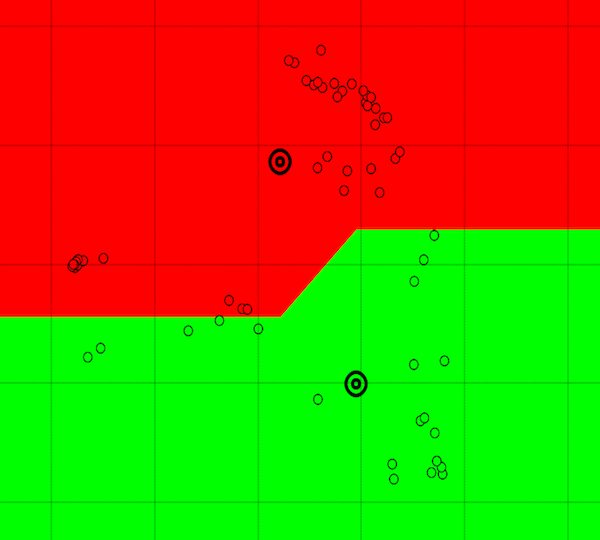
\includegraphics[height=0.14\textheight]{./clustering/l1norm.png}
	\caption{\bf Manhattan}
	\end{subfigure}
    \begin{subfigure}[h]{0.23\textwidth}
    \centering
    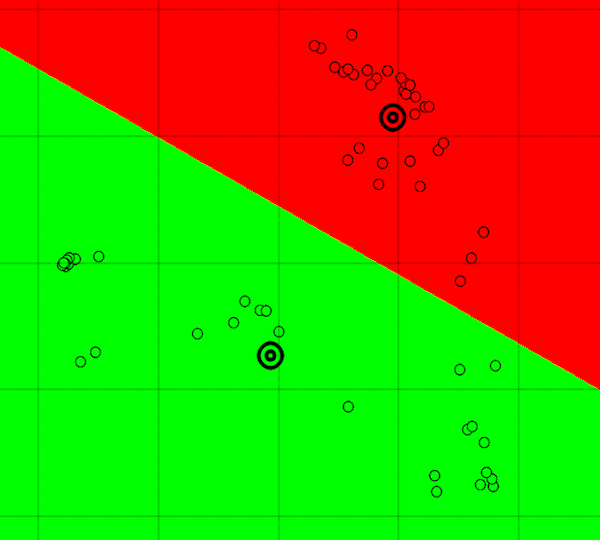
\includegraphics[height=0.14\textheight]{./clustering/l2norm.png}
	\caption{\bf Euclidean}
    \end{subfigure}
    \begin{subfigure}[h]{0.23\textwidth}
    \centering
   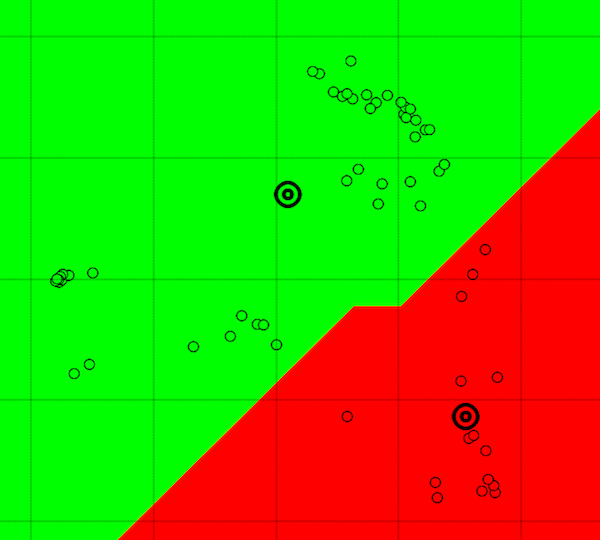
\includegraphics[height=0.14\textheight]{./clustering/l0norm.png}
	\caption{\bf Infinity}
    \end{subfigure}
    \begin{subfigure}[h]{0.23\textwidth}
    \centering
    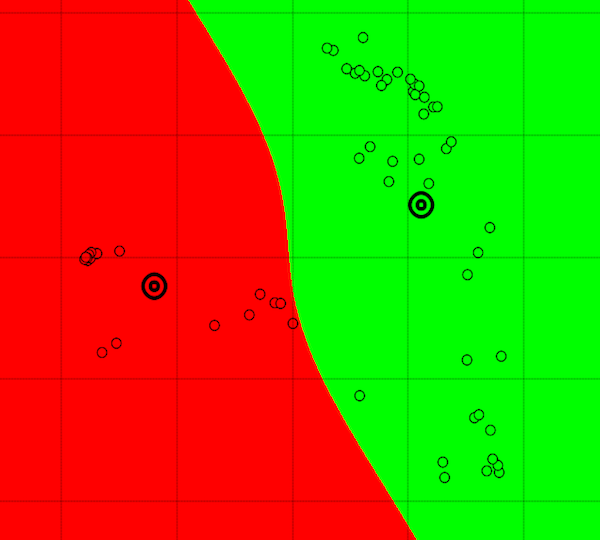
\includegraphics[height=0.14\textheight]{./clustering/lpnorm.png}
	\caption{\bf Polynomial}
    \end{subfigure}
\caption{K-means clustering method with different metrics}
\label{fig:figure4}
\end{figure}
\subsubsection{Soft K-means method}
The soft K-means technique has an another hyperparameter called $\beta$, it represents the stiffness of the borders. This parameter is also related to the disparity across clusters (inversely proportional to $\beta$). The responsibility of each sample is a real number varying between 0 and 1. For each iteration of the algorithm, the centroids are adjusted to match the weighted means of the data points that they are responsible for.
In other words, the sample which are between two clusters will have less responsibility in the soft K-means method than hard K-means method.\\
In our case, we found that a value of 10 for $\beta$ gives a fairly good clustering. In fact, with a $\beta$ of 4, the disparity in the cluster is high. Consequently, the algorithm found only 1 cluster. Furthermore, the higher the $\beta$ value is, the more the Soft-K-Means results looks like the standard method as we can see on \ref{fig:figure5} with a $\beta$ equals to 100.

\begin{figure}[!h]
\centering
	\begin{subfigure}[h]{0.30\textwidth}
    \centering
	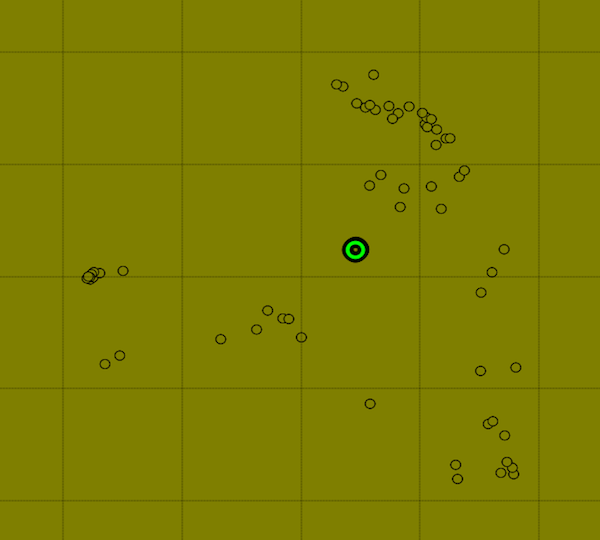
\includegraphics[height=0.13\textheight]{./clustering/soft_k_mean_beta_4.png}
	\caption{$\boldsymbol \beta \bf = 4$}
	\end{subfigure}
    \begin{subfigure}[h]{0.30\textwidth}
    \centering
    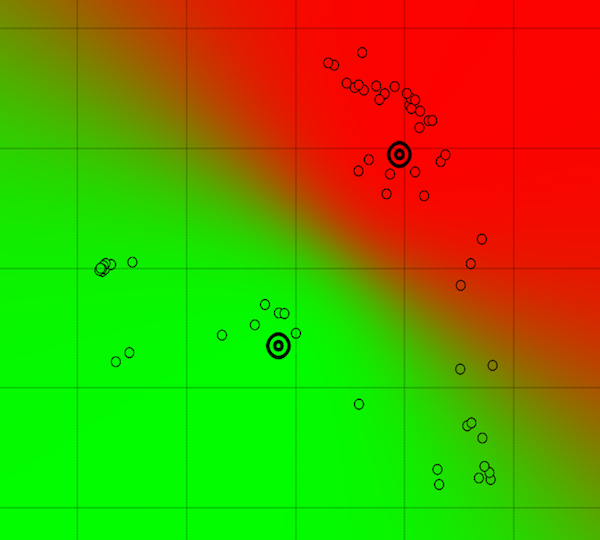
\includegraphics[height=0.13\textheight]{./clustering/soft_k_mean_beta_10.png}
	\caption{$\boldsymbol \beta \bf = 10$}
    \end{subfigure}
    \begin{subfigure}[h]{0.30\textwidth}
    \centering
    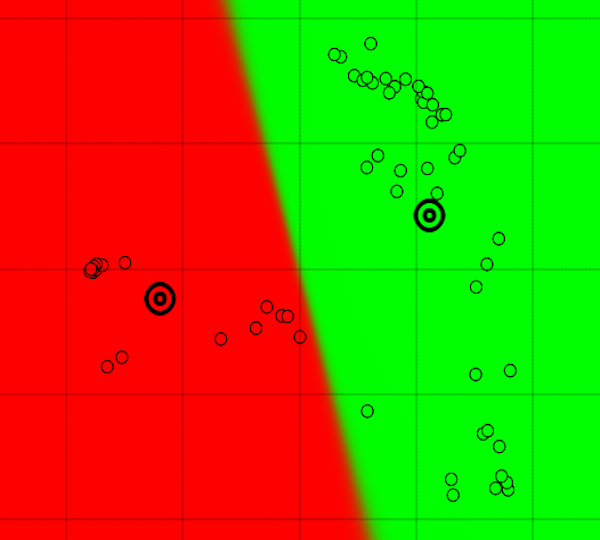
\includegraphics[height=0.13\textheight]{./clustering/soft_k_mean_beta_100.png}
	\caption{$\boldsymbol \beta \bf = 100$}
    \end{subfigure}
\caption{Soft K-means clustering method with different values of $\beta$}
\label{fig:figure5}
\end{figure}

\subsubsection{DBSCAN method}
%test avec mesure cosine pour checker les neighboor par rapport à l'angle, mais ça ne donne rien
In this method, there are 2 hyperparameters $\epsilon$ and $m_{data}$. The variable $\epsilon$ characterized the size of the neighborhood and $m_{data}$ the minimum number of data points required to consider the group of points as a cluster. If the size of neighborhood $\epsilon$ is too high, the algorithm may merged different closed clusters into one. Thus, the risk is to have less cluster than expected if the data points are not well separated. However, if the $\epsilon$ is too low, the algorithm may detect more outliers and more clusters.Hence, data points won't be well clustered as we can see on figure \ref{fig:figure6}. In our case, we found that a value of 0.230 for $\epsilon$, results in a satisfactory clustering. 

\begin{figure} [ht]
\centering
	\begin{subfigure}[h]{0.30\textwidth}
    \centering
	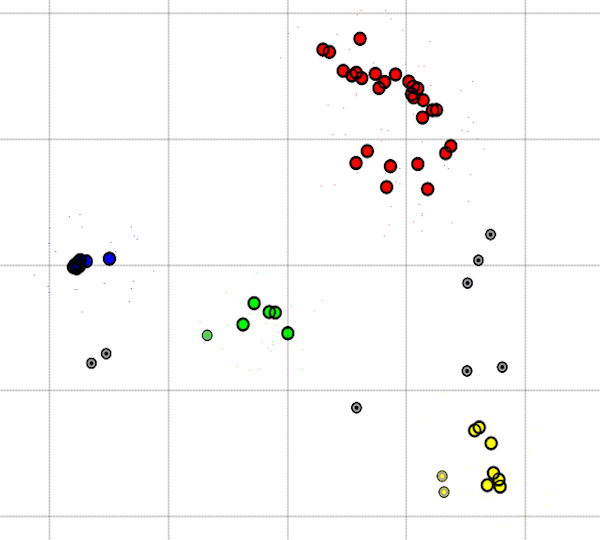
\includegraphics[height=0.18\textheight]{./clustering/dbs_scan_eps_0100_min_3.png}
	\caption{$\boldsymbol \epsilon \bf= 0.100$}
	\end{subfigure}
    \begin{subfigure}[h]{0.30\textwidth}
    \centering
    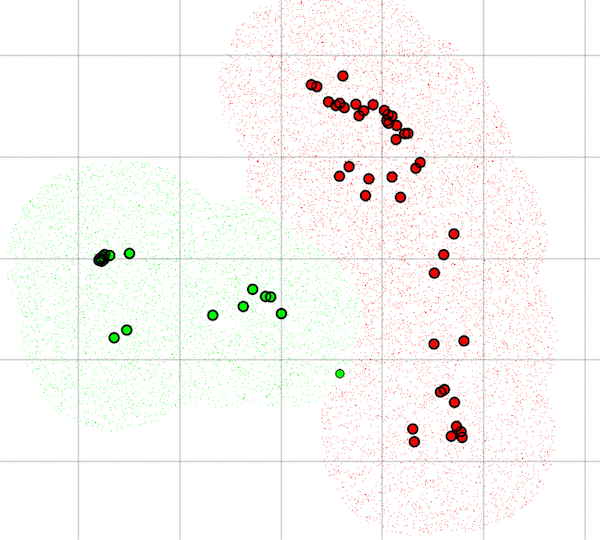
\includegraphics[height=0.18\textheight]{./clustering/dbs_scan_eps_0230_min_3.png}
	\caption{$\boldsymbol \epsilon \bf = 0.230$}
    \end{subfigure}
    \begin{subfigure}[h]{0.30\textwidth}
    \centering
    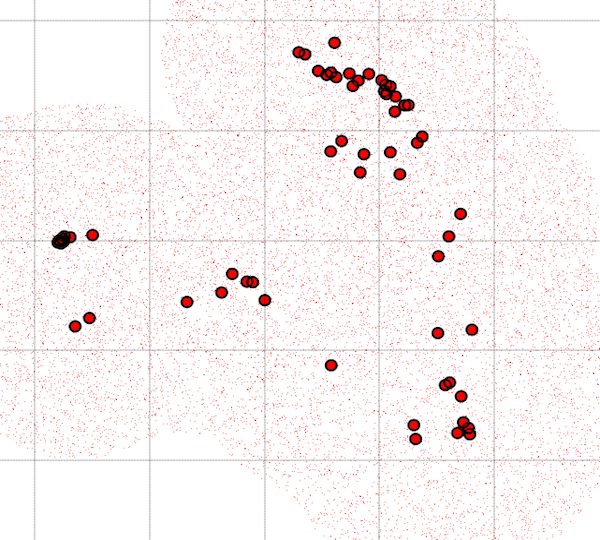
\includegraphics[height=0.18\textheight]{./clustering/dbs_scan_eps_0300_min_3.png}
	\caption{$\boldsymbol \epsilon \bf = 0.300$}
    \end{subfigure}

\caption{Influence of $\epsilon$ parameter on DBSCAN method}
\label{fig:figure6}
\end{figure}

\subsection{Quantitative assessment}

In this section, we will perform K-Means and Soft-K-Means clustering methods and looking at different metrics. If we optimized the algorithm regarding the RSS, we always found a large number of cluster as a result as we can see on figure \ref{fig:figure7}. The higher is the number of cluster K, the lower is the RSS value. Thus, it is not relevant to optimize regarding the RSS because at the end, it will have more cluster than expected. 

\begin{figure} [ht]
\centering
	\begin{subfigure}[h]{0.45\textwidth}
    \centering
	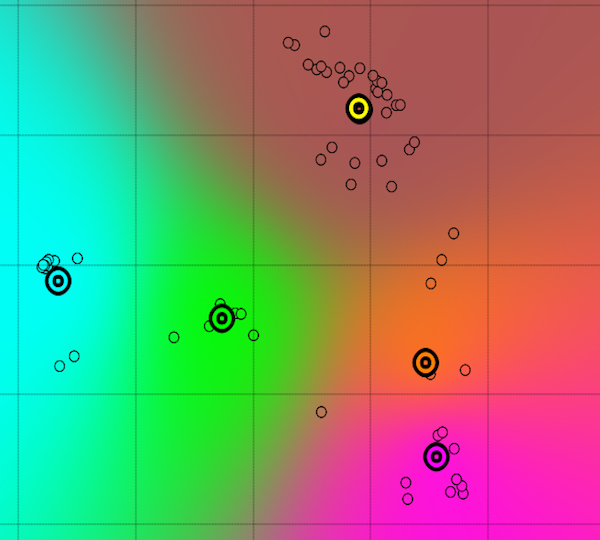
\includegraphics[height=0.15\textheight]{./clustering/opt_RSS_k_soft_beta_10_range8.png}
	\caption{\bf Soft K-means ($\boldsymbol \beta \bf = 10$ - range [0,8])}
	\end{subfigure}
    \begin{subfigure}[h]{0.45\textwidth}
    \centering
    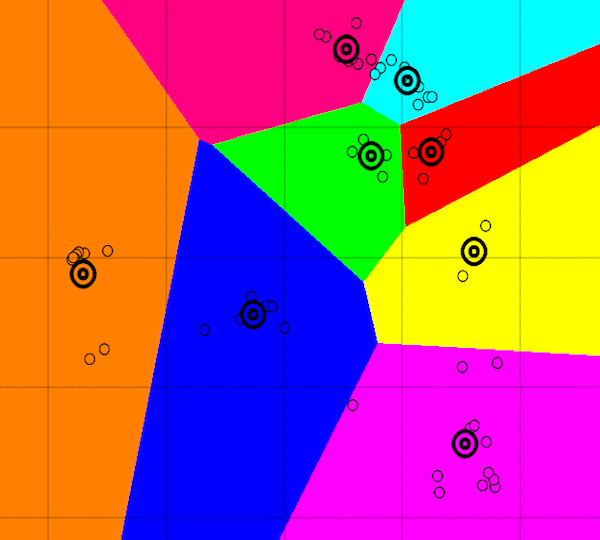
\includegraphics[height=0.15\textheight]{./clustering/opt_RSS_k_mean_L2_range8.png}
	\caption{\bf K-means (norm L2 - range [0,8])}
    \end{subfigure}
\caption{Results of optimization regarding RSS}
\label{fig:figure7}
\end{figure}

Once we optimized the algorithm with respect to a specific metric (BIC-AIC), we generally get 3 clusters as we can see on the figure \ref{fig:figure8}. It can be explained by the distribution of the points which are sparse.

\begin{figure} [ht]
\centering
	\begin{subfigure}[t]{0.25\textwidth}
    \centering
	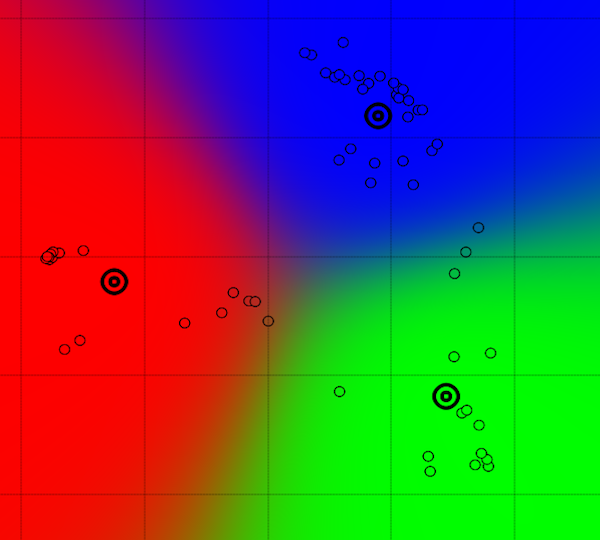
\includegraphics[height=0.15\textheight]{./clustering/opt_AIC_k_soft_beta_10_range7.png}
	\caption{\bf Soft K-means - $\boldsymbol \beta \bf=10$}
	\end{subfigure}
    \hspace{20mm}
    \begin{subfigure}[t]{0.50\textwidth}
	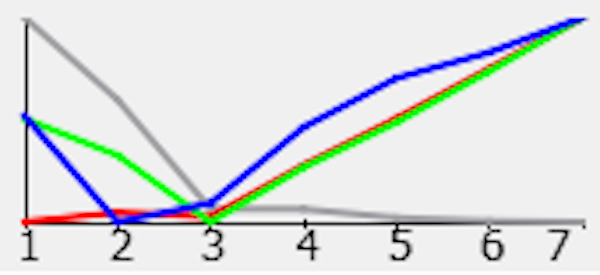
\includegraphics[height=0.15\textheight,right]{./clustering/curve_opt_AIC_k_soft_beta_10_range7.png}
	\caption{\bf Curve of optimization - Soft K-means $\boldsymbol \beta \bf = 10$. (\textcolor{gray}{RSS}, \textcolor{red}{BIC}, \textcolor{green}{AIC} and \textcolor{blue}{F1-Measure})}
	\end{subfigure}\\
    \begin{subfigure}[t]{0.25\textwidth}
    \centering
    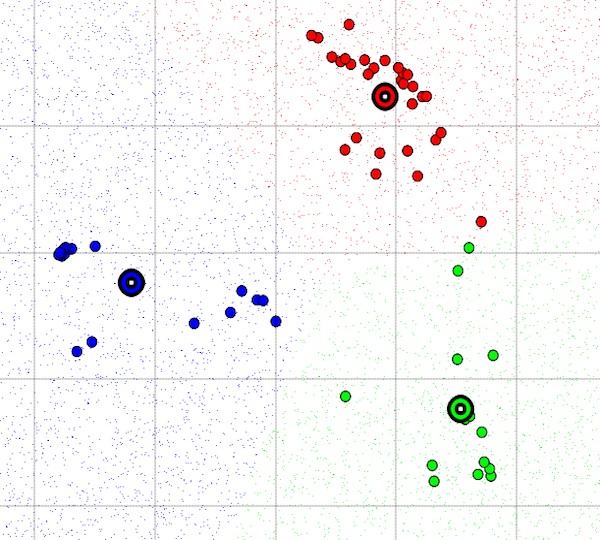
\includegraphics[height=0.15\textheight, right]{./clustering/opt_AIC_k_mean_L2_range5.png}
	\caption{\bf K-means - norm L2}
    \end{subfigure} 
    \hspace{20mm}
    \begin{subfigure}[t]{0.50\textwidth}
    \centering
    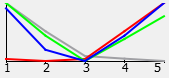
\includegraphics[height=0.15\textheight]{./clustering/curve_opt_AIC_k_mean_L2_range5.png}
	\caption{\bf Curve of optimization - K-means norm L2. (\textcolor{gray}{RSS}, \textcolor{red}{BIC}, \textcolor{green}{AIC} and \textcolor{blue}{F1-Measure})}
    \end{subfigure}
\caption{Results of optimization regarding AIC}
\label{fig:figure8}
\end{figure}

Yet, optimizing regarding to the BIC allowed to get 2 clusters but the hyperparameter has to be well-tuned as we can see on the figure \ref{fig:figure9} especially in the case of Soft K-means with $\beta$. In our case, penalizing the likelihood with the number of free parameters with the number of data points (BIC) give results more favorable than penalizing only with the number of free parameter (AIC). 

\begin{figure} [h]
\centering
	\begin{subfigure}[t]{0.25\textwidth}
    \centering
	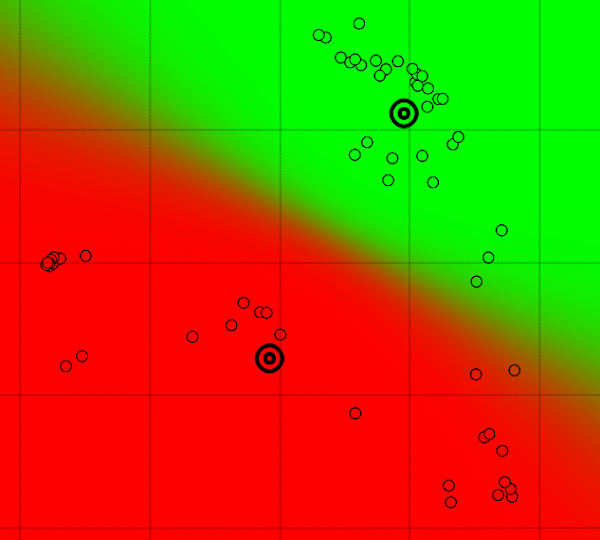
\includegraphics[height=0.15\textheight]{./clustering/opt_BIC_k_soft_beta_20_range7.png}
	\caption{\bf Soft K-means - $\boldsymbol \beta \bf = 10$}
	\end{subfigure}
    \hspace{20mm}
    \begin{subfigure}[t]{0.50\textwidth}
    \centering
	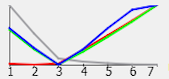
\includegraphics[height=0.15\textheight]{./clustering/curve_opt_BIC_k_soft_beta_20_range7.png}
	\caption{\bf Curve of optimization - Soft K-means $\boldsymbol \beta \bf = 20$. (\textcolor{gray}{RSS}, \textcolor{red}{BIC}, \textcolor{green}{AIC} and \textcolor{blue}{F1-Measure})}
	\end{subfigure}\\
    \begin{subfigure}[t]{0.25\textwidth}
    \centering
    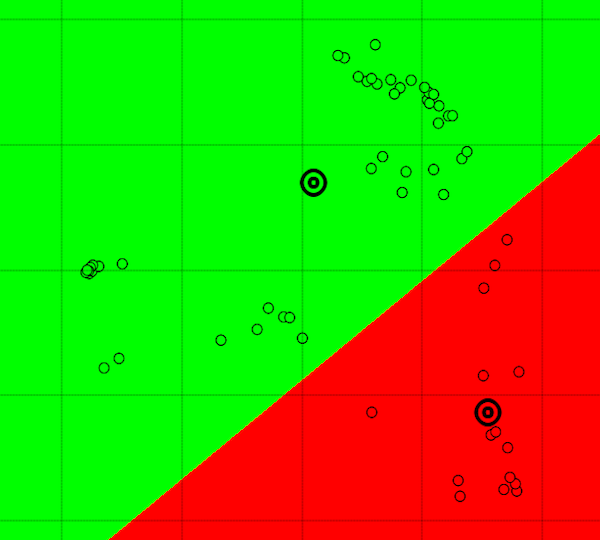
\includegraphics[height=0.15\textheight]{./clustering/opt_BIC_k_mean_L2_range5.png}
	\caption{\bf K-means - norm L2}
    \end{subfigure}
    \hspace{20mm}
    \begin{subfigure}[t]{0.50\textwidth}
    \centering
    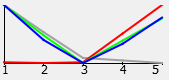
\includegraphics[height=0.15\textheight]{./clustering/curve_opt_BIC_k_mean_L2_range5.png}
	\caption{\bf Curve of optimization - K-means norm L2. (\textcolor{gray}{RSS}, \textcolor{red}{BIC}, \textcolor{green}{AIC} and \textcolor{blue}{F1-Measure})}
    \end{subfigure}
\caption{Results of optimization regarding BIC}
\label{fig:figure9}
\end{figure}


In this part, we will evaluate the semi-supervised learning on our dataset. We vary the percentage of labeled data going from very low ratio to high ratios and optimize with respect to F1-measure.

With the soft-K-means method and 10\% of the data labeled, we obtained 3 clusters (\ref{fig:figure10a}) whereas we expected only 2 but the F1-measure is equal to 0.90, close to 1. If we increased the ratio to 50\% the algorithm is able to separate the data into 2 clusters (\ref{fig:figure10b}) and we have a good F1-measure of 0.91. 

\begin{figure}[h]
\centering
	\begin{subfigure}[h]{0.25\textwidth}
    \centering
	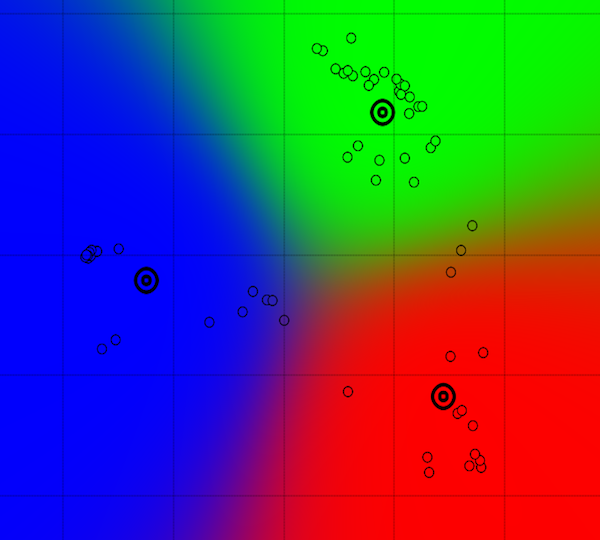
\includegraphics[height=0.15\textheight]{./clustering/opt_F1_10__soft_k__beta_10_range7.png}
	\caption{$\boldsymbol \beta \bf = 10$\bf, 10\% labeled}
    \label{fig:figure10a}
	\end{subfigure}
    \hspace{20mm}
    \begin{subfigure}[h]{0.50\textwidth}
    \centering
	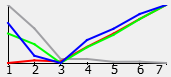
\includegraphics[height=0.15\textheight]{./clustering/curve_opt_F1_10__soft_k__beta_10_range7.png}
	\caption{\bf Curve of optimization - $ \boldsymbol \beta \bf = 10$ - 10\% labeled. (\textcolor{gray}{RSS}, \textcolor{red}{BIC}, \textcolor{green}{AIC} and \textcolor{blue}{F1-Measure})}
    \label{fig:figure10c}
	\end{subfigure}\\
    \begin{subfigure}[h]{0.25\textwidth}
    \centering
    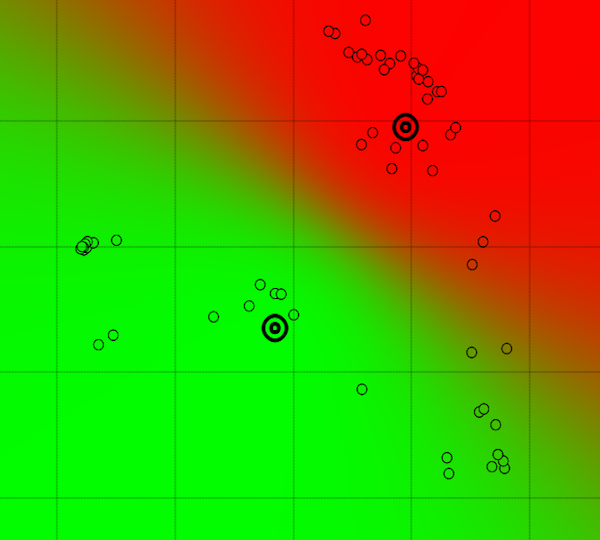
\includegraphics[height=0.15\textheight]{./clustering/opt_F1_50__soft_k__beta_10_range7.png}
	\caption{$\boldsymbol \beta \bf = 10$\bf, 50\% labeled}
    \label{fig:figure10b}
    \end{subfigure}
    \hspace{20mm}
    \begin{subfigure}[h]{0.50\textwidth}
    \centering
    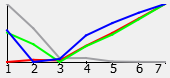
\includegraphics[height=0.15\textheight]{./clustering/curve_opt_F1_50__soft_k__beta_10_range7.png}
	\caption{\bf Curve of optimization - $\boldsymbol \beta \bf = 10$ - 50\% labeled. (\textcolor{gray}{RSS}, \textcolor{red}{BIC}, \textcolor{green}{AIC} and \textcolor{blue}{F1-Measure})}
    \label{fig:figure10d}
    \end{subfigure}
\caption{Soft K-means - results of optimization regarding F1}
\label{fig:figure10}
\end{figure}

With the standard k-means method, in our case, the algorithm is not able to well-clustered the data points (\ref{fig:figure11a}) with 50\% of the dataset labeled. It needs 100\% to get 2 clusters (\ref{fig:figure11b}) at the end. Thus, this algorithm is not relevant in this problem because it costs a lot in terms of data labeled. 

\begin{figure}[h]
\centering
	\begin{subfigure}[h]{0.25\textwidth}
    \centering
	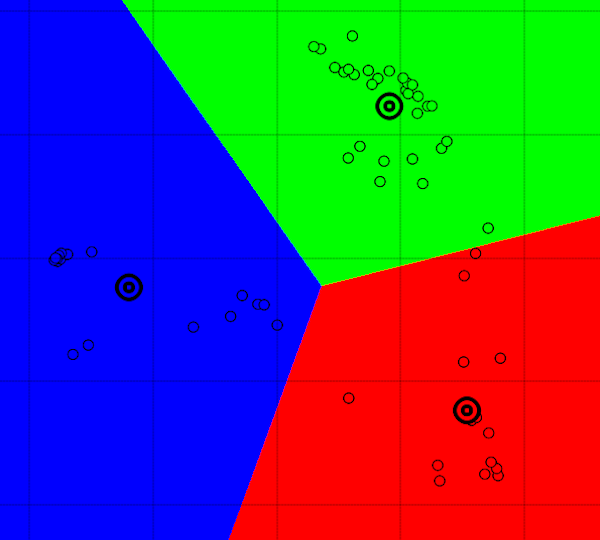
\includegraphics[height=0.15\textheight]{./clustering/opt_F1_50__k_mean_L2_range7.png}
	\caption{\bf L2 norm - 50\% labeled}
    \label{fig:figure11a}
	\end{subfigure}
    \hspace{20mm}
	\begin{subfigure}[h]{0.50\textwidth}
    \centering
	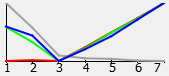
\includegraphics[height=0.15\textheight]{./clustering/curve_opt_F1_50__k_mean_L2_range7.png}
	\caption{\bf Curve of optimization - L2 norm - 50\% labeled. (\textcolor{gray}{RSS}, \textcolor{red}{BIC}, \textcolor{green}{AIC} and \textcolor{blue}{F1-Measure})}
    \label{fig:figur11c}
	\end{subfigure}\\ 
    \begin{subfigure}[h]{0.25\textwidth}
    \centering
    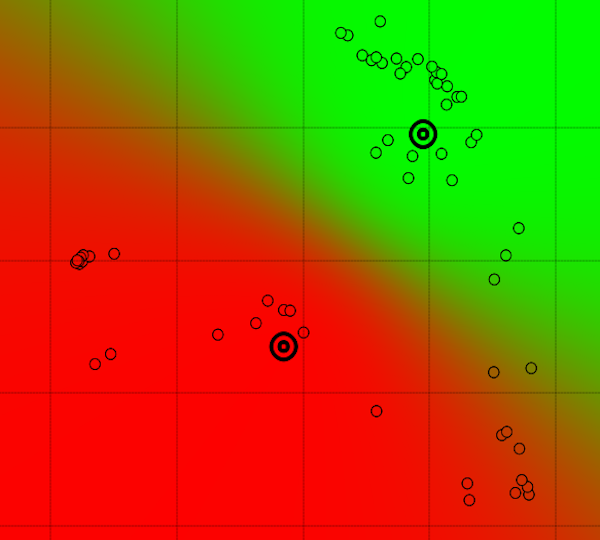
\includegraphics[height=0.15\textheight]{./clustering/opt_F1_100__k_mean_L2_range7.png}
	\caption{\bf L2 norm - 100\% labeled}
    \label{fig:figure11b}
    \end{subfigure}
    \hspace{20mm}
    \begin{subfigure}[h]{0.50\textwidth}
    \centering
    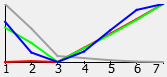
\includegraphics[height=0.15\textheight]{./clustering/curve_opt_F1_100__k_mean_L2_range7.png}
	\caption{\bf Curve of optimization - L2 norm - 100\% labeled. (\textcolor{gray}{RSS}, \textcolor{red}{BIC}, \textcolor{green}{AIC} and \textcolor{blue}{F1-Measure})}
    \label{fig:figure11d}
    \end{subfigure}
\caption{\bf K-means - results of optimization regarding F1}
\label{fig:figure11}
\end{figure}


